\documentclass[runningheads]{llncs}
\usepackage[T1]{fontenc}
\usepackage[utf8]{inputenc}
\usepackage{booktabs}
\usepackage{graphicx}
\usepackage{xcolor}
\usepackage[hidelinks]{hyperref}
\hypersetup{pdftitle={Puno Quechua ASR: When to Adapt the Speech Encoder, and Verification as the Bottleneck},
  pdfauthor={Irving Ernesto Quezada Ram\'irez}}
\emergencystretch=1em
\newcommand{\ci}[2]{$[#1,#2]$}  % 95% bootstrap interval

\begin{document}
\title{Puno Quechua ASR: When to Adapt the Speech Encoder, and Verification as the Bottleneck}
\titlerunning{Puno Quechua ASR with Provided Data Only}
\author{Irving Ernesto Quezada Ram\'irez}
\authorrunning{I. E. Quezada Ram\'irez}
\institute{Independent Researcher\\
\email{research@irvingernesto.com}}
\maketitle

\begin{abstract}
We describe our system for Task~1 of the SIMBig 2026 shared task, Puno Quechua (qxp) ASR from the
provided data and public models only, with four findings. (1)~The official splits reuse every
prompt sentence between training and test, which can reverse the ranking of systems; we evaluate
on held-out sentences, speakers and an out-of-domain (OOD) radio drama. (2)~Hybrid rescoring of
LLM-ASR, CTC and perturbed-audio candidates reaches 14.1\% WER on the radio drama vs.\ 20.9\%
for the best of 37 public checkpoints. (3)~LoRA on the speech encoder instead of the LLM decoder
cuts WER on new sentences by 3.7 points for omniASR-LLM-7B and by 6.4 and 4.6 for two Whisper seeds
(the second n.s.), not for smaller omniASR encoders, which encode Quechua stop
contrasts almost as well. In the 7B, the gain needs the lower layers, survives truncation to 4 of
16 singular directions per projection, and leaves the N-best oracle unchanged while ranking
candidates better. (4)~Verification is the bottleneck: sampling and perturbed audio propose better
transcripts than beam search, but our reranker orders candidate pairs correctly only 71--78\%
of the time.
\end{abstract}
\keywords{Speech recognition \and Quechua \and LLM-ASR \and LoRA \and Reranking}

\section{Introduction}
The Puno region of southern Peru has about 474{,}000 native Quechua speakers (2017 census)
\cite{huaman2025cv}.
Earlier Quechua ASR targeted Southern Quechua
\cite{cardenas2018siminchik,zevallos2022augment}; Common Voice now provides 30.5\,h of read and
5\,h of spontaneous Puno Quechua \cite{ardila2020cv,huaman2025cv}, on which the organizers fine-tune
XLS-R \cite{babu2022xlsr,huaman2026community}; MMS \cite{pratap2024mms} covers related Quechua
varieties, and Omnilingual ASR \cite{omnilingual2025} supports qxp out of the box (\emph{zero-shot}
below: without our fine-tuning). EAVA \cite{shi2026eava} argued, with gains on children's and dialectal speech, that
adapting only the LLM leaves the encoder under-adapted; we ask when this holds, across encoder sizes and
model families, and what the encoder update changes (Fig.~\ref{fig:where}). Both analyses end at
ranking: encoder adaptation helps the 7B rank candidates, and ranking limits our full system. We contribute:
\begin{enumerate}
\item \emph{A held-out-sentence evaluation:} prompt reuse makes a prompt 4-gram best on seen
sentences and worse than no LM on new ones (Sect.~\ref{sec:data}).
\item \emph{A system} that beats all 37 public checkpoints out of domain (Sect.~\ref{sec:system},~\ref{sec:results}).
\item \emph{Where to adapt an LLM-ASR model:} the encoder for omniASR-LLM-7B and Whisper, not for
smaller omniASR encoders; in the 7B, the gain needs the bottom encoder quarter, survives
truncation to 4 of 16 directions, and ranks the same candidates better (Sect.~\ref{sec:where}).
\item \emph{Verification is the bottleneck:} ranking, not candidates, limits WER
(Sect.~\ref{sec:rl}).
\end{enumerate}

\begin{figure}[t]
\centering
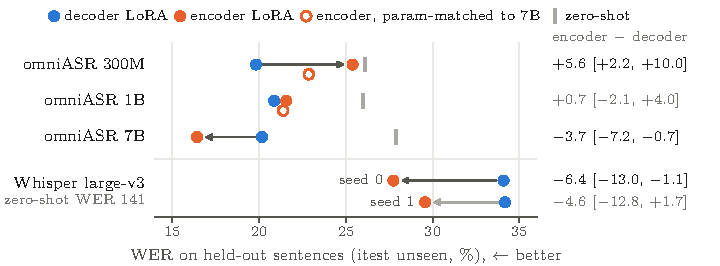
\includegraphics{figs/where_to_adapt.pdf}
\caption{\textbf{Adapting the encoder instead of the decoder helps only omniASR-7B and
Whisper.} Itest-unseen WER; hollow: encoder LoRA with the 7B's parameter count (rank 160/64).
Right: encoder $-$ decoder, 95\% interval, grey if it includes 0. Whisper: clips $\le$30\,s.}
\label{fig:where}
\end{figure}

\section{Sentence Reuse Reverses the Ranking of Systems}\label{sec:data}
\paragraph{Data.} Scripted Speech 27.0 provides 22{,}727 validated clips (30.5\,h, 77 speakers)
over only 2{,}051 distinct sentences. Spontaneous Speech 5.0 provides 1{,}074 gold transcriptions
(5.2\,h, 20 speakers); 5{,}651 untranscribed clips have organizer ``silver'' labels from
omniASR-LLM-7B. The shared-task test (659 clips) reads new sentences:
zero-shot hypotheses of its 438 scripted clips lie as far from the closest training prompt as
held-out sentences do (median normalized edit distance 0.495 vs.\ 0.489; seen sentences 0.028).
Its 221 spontaneous clips come from speakers aged 60+; 1{,}069 of the 1{,}074 gold clips, from
speakers under 40.

\paragraph{Protocol.} Scripted dev and internal test (\emph{itest}) are the organizers' dev and
test splits (21+21 speakers). We hold out 400 sentences from all training audio and text; their
dev/itest clips form the \emph{unseen} subsets. Spontaneous dev/itest are the gold clips of the
official dev/test speakers (4 and 6), whose other clips are not trained on. \emph{OOD} is the
organizers' 109-clip radio drama. \emph{Dev-mode} models train on none of these; submitted
\emph{final-mode} models also train on itest and held-out sentences. Weights are tuned on dev
(OOD informed three decisions).

\paragraph{The public splits reward memorization.} The organizers' splits share all
scripted sentences between training and test. On seen
sentences, CTC with a word 4-gram on the training prompts beats our system (dev/itest WER
6.0/7.5 vs.\ 10.0/11.9); on held-out sentences it is worse than without the LM (18.7/25.0 vs.\
14.6/21.3; dev $+4.0$ \ci{+0.9}{+7.2}, itest $p{=}0.051$) and ours wins (9.7/16.9). The LM's seen-minus-held-out effect is $-12.1$
\ci{-18.0}{-7.1} points on dev, $-12.9$ \ci{-18.7}{-7.3} on itest. Like the official test, we
select systems on held-out sentences.

\begin{table}[t]
\caption{\textbf{Decoder adaptation generalizes to new sentences and out of domain; encoder
adaptation and rescoring add gains on new sentences.} WER (\%), provided data only, dev-mode
systems unless noted. $^\dagger$Hybrid tuning set.}
\label{tab:main}
\centering\footnotesize
\setlength{\tabcolsep}{3.5pt}
\begin{tabular}{lccccc}
\toprule
& dev & itest & dev & itest & \\
System & unseen$^\dagger$ & unseen & spont$^\dagger$ & spont & OOD \\
\midrule
omniASR-LLM-7B zero-shot & 21.3 & 27.9 & 14.3 & 7.3 & 23.3 \\
CTC-1B, soup + WiSE-FT & 14.6 & 21.3 & 19.1 & 8.2 & 19.3 \\
LLM-7B, decoder LoRA, silver labels (v1) & 12.6 & 20.2 & 14.8 & 6.8 & 14.9 \\
LLM-7B, decoder LoRA, self-trained (v2) & 13.1 & 20.2 & 14.9 & 6.6 & 15.1 \\
LLM-7B, encoder LoRA & 11.7 & 16.4 & 14.8 & 6.7 & 15.0 \\
LLM-7B, enc+dec LoRA & 10.9 & 16.0 & 14.6 & 6.8 & 15.4 \\
\midrule
Hybrid rescoring (zero-shot, v1, v2, CTC) & 9.8 & 17.4 & 13.7 & \textbf{6.2} & 14.5 \\
\quad + perturbed views (full system) & 9.7 & 16.9 & \textbf{13.5} & \textbf{6.2} & 13.7 \\
\quad + enc+dec LoRA as scorer & \textbf{9.2} & \textbf{15.5} & \textbf{13.5} & \textbf{6.2} &
\textbf{13.4} \\
\midrule
Submission (final mode) & -- & -- & 13.8$^\dagger$ & -- & 14.1 \\
\bottomrule
\end{tabular}
\end{table}

\paragraph{Statistics.} Paired bootstraps of corpus-WER differences \cite{bisani2004bootstrap}
(10{,}000 resamples; 95\% intervals) resample speakers $\times$ sentences on read
speech (pigeonhole bootstrap \cite{owen2007pigeonhole}) and clips elsewhere; spontaneous results
(4 and 6 speakers) are descriptive. Two confirmatory hypotheses, designated post hoc
(not preregistered) and Holm-corrected \cite{holm1979} on itest unseen and OOD: the \emph{full
system} beats its best dev-unseen component, LoRA v1; perturbed views help. Other intervals are
unadjusted.

\section{A System Built from Provided Data Only}\label{sec:system}
\paragraph{CTC branch.} We fine-tune omniASR-CTC-1B-v2 (frozen CNN, masking \cite{park2019specaugment},
speed and noise augmentation \cite{ko2015augment}; 12k updates of 200\,s) and interpolate the average of its last four checkpoints
with the zero-shot weights (WiSE-FT \cite{wortsman2022wiseft},
$\alpha{=}0.85$).

\paragraph{LLM-ASR branch.} omniASR-LLM-7B-v2 feeds a 7B wav2vec~2.0 encoder
\cite{baevski2020wav2vec} into a LLaMA decoder. \emph{Decoder LoRA} trains rank-16 adapters
\cite{hu2022lora} on all decoder projections, encoder frozen (lr $3{\cdot}10^{-4}$,
1{,}200--1{,}500 updates of 240\,s): \emph{v1} on the silver labels, \emph{v2} on our
pseudo-labels. \emph{Encoder LoRA} adapts all encoder projections, decoder frozen;
\emph{enc+dec} adapts both (v2 data, lr $2{\cdot}10^{-4}$). Pseudo-labels come from ROVER \cite{fiscus1997rover} of v1,
the CTC model and the silver labels, kept at $\le$15\% disagreement (27.5\,h).

\paragraph{Hybrid rescoring.} As in hybrid CTC/attention decoding \cite{watanabe2017hybrid}, each
clip's candidates (16-best of a pyctcdecode beam search with a word 4-gram KenLM \cite{heafield2011kenlm};
beam-8 N-best of the zero-shot model, v1 and v2) are scored by $\log P_{\mathrm{CTC}}(y\mid x)$
plus a weighted sum of a character 10-gram, length and every LLM adapter's log-likelihood
(weights: random search on dev). LMs use in-domain text only.

\paragraph{Perturbed-view candidates.} The zero-shot model and v2 also greedily decode six
perturbed copies of each clip (speed 0.85--1.1, 15--20\,dB noise); new candidates are scored on
the \emph{original} audio, plus a view-count feature (cf.\ test-time augmentation
\cite{jelea2025gtta}).

\section{Results: Best Out of Domain Among Public Systems}\label{sec:results}

\paragraph{Confirmatory tests.} The full system beats v1 on itest unseen ($-3.3$
\ci{-6.5}{-0.8}, Holm-adjusted $p{=}0.04$); on OOD its gain ($-1.2$ \ci{-2.4}{-0.2}) fails the
correction ($p{=}0.12$). The views are not significant ($-0.5$ \ci{-1.8}{0.0},
$-0.8$ \ci{-1.8}{+0.1}), though negative on every read and OOD set in all weight searches.

\paragraph{Adaptation gives the largest gain, rescoring the next} (Table~\ref{tab:main}). Decoder
LoRA helps on new sentences and out of domain (v1 vs.\ zero-shot: itest unseen $-7.7$
\ci{-11.8}{-4.6}, OOD $-8.4$ \ci{-10.7}{-6.0}), not on young-speaker spontaneous sets;
rescoring improves on its best component, v1 (itest unseen $-2.8$ \ci{-5.7}{-0.4}).
Two more v2 seeds move WER by up to 1.2 (OOD): training noise.
Enc+dec LoRA beats v2 on itest unseen in both seeds ($-4.2$ \ci{-7.3}{-1.5}, $-4.9$
\ci{-8.4}{-1.9}), not on spontaneous or OOD; as the submission's fourth scorer it changes the
hybrid by $-1.4$ \ci{-3.1}{+0.2} on itest unseen (n.s.).

\paragraph{Out of domain, the system beats every public checkpoint.} On the radio drama, the best
of 37 public qxp models (listed in our repository; greedy) is omniASR-LLM-1B-v2 zero-shot
(20.9/2.9 WER/CER), the best organizer one (\mbox{XLS-R-300M}) 24.5/4.1, our submission (not
compute-matched) 14.1/2.3 ($-6.7$ \ci{-9.2}{-4.4}).

\section{Where Should an LLM-ASR Model Be Adapted?}\label{sec:where}
\paragraph{The encoder for the 7B and Whisper, not for the smaller omniASR encoders.} The omniASR-LLM models
with 300M, 1B and 7B encoders share one decoder (v2 data and recipe, rank 16, one seed unless
noted). Encoder LoRA beats decoder LoRA for the 7B and Whisper large-v3
\cite{radford2023whisper}, whose decoder knows no Quechua (Fig.~\ref{fig:where}, seed 1 n.s.; Whisper OOD
$-8.8$ and $-7.6$, both significant), not for the 300M or 1B. With as many parameters as the 7B's
encoder LoRA (rank 160 on the 300M, 64 on the 1B), encoder LoRA improves the 300M (25.4$\rightarrow$22.9) but still trails
decoder LoRA ($+3.0$ \ci{-0.1}{+6.3}; 1B $+0.5$ \ci{-2.5}{+4.0}); the learning rate was tuned
at 7B. Decoder LoRA brings all three sizes to about 20\% (19.8, 20.9, 20.2; zero-shot
26.1, 26.0, 27.9); only the 7B encoder adds to that. Untested hypotheses: the omniASR decoder
already knows qxp (LLM LoRA acts through linguistic priors \cite{kolluri2026depth}), unlike
Whisper's, and only the 7B encoder changes enough.

\paragraph{The information is there; the encoders move differently.} Linear probes trained on dev
and tested on itest speakers separate ejective from plain, aspirated from plain and /q/ from /k/ at
94--97\% in all three pretrained encoders (Fig.~\ref{fig:plasticity}a; shuffled-label controls
\cite{hewitt2019control} near 50\%); adaptation adds up to 1--2 points in the 7B's upper layers. What differs
is how far adaptation moves the encoder: the 300M and 1B keep a linear CKA \cite{kornblith2019cka}
$\ge$0.97 to the pretrained encoder up to about 80\% depth, the 7B drops to 0.84 by layer 16 of
128 (Fig.~\ref{fig:plasticity}b). Descriptive and confounded: the 7B uses the enc+dec adapter, the others 4--10 times smaller
encoder adapters; two 7B seeds differ more from each other (0.65) than from the pretrained one.

\begin{figure}[t]
\centering
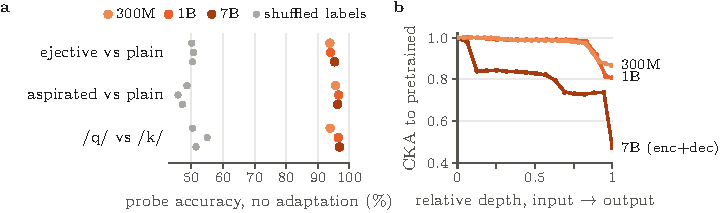
\includegraphics{figs/plasticity.pdf}
\caption{\textbf{Every encoder already separates the stop contrasts; adaptation moves the 300M
and 1B only near the top, the 7B (enc+dec) from an eighth of its depth.} (a)~Best-layer probe
accuracy of the pretrained encoders on force-aligned stops, held-out speakers. (b)~Linear CKA to
the pretrained encoder (dev frames).}
\label{fig:plasticity}
\end{figure}

\paragraph{The read-speech gain needs the lower layers, and four directions suffice.} Zeroing the
top quarter of the trained 7B encoder update, where fine-tuning changes wav2vec~2.0 most
\cite{pasad2021layerwise}, has no detectable effect ($-0.3$ \ci{-1.6}{+1.0}); zeroing the bottom
quarter costs $+3.7$ \ci{+1.0}{+7.3}, about the whole gain over decoder LoRA; both enc+dec seeds
agree (Fig.~\ref{fig:layers}a). The bottom quarter is necessary but not sufficient (alone 22.4); an adapter trained on the bottom
half matches one trained on all layers (16.1 vs.\ 16.4; top half 20.6). Out of domain (descriptive), zeroing
the bottom quarter does not hurt (14.3 vs.\ 15.0) and layers 32--63 alone keep the gain over
zero-shot (15.3 vs.\ 23.3; enc+dec seeds: 16.2 vs.\ 15.4, 15.0). Per projection, the top
four of 16 singular directions hold 85\% of the update's squared Frobenius norm and keep the whole gain
(Fig.~\ref{fig:layers}b; cf.\ \cite{aghajanyan2021intrinsic}); keeping 2 or 1 costs a
non-significant $+0.6$ or $+1.4$. Two seeds' top-4 subspaces barely overlap
($\|U_1^\top U_2\|_F^2/4{=}0.02$--$0.08$; 1 = identical).

\begin{figure}[t]
\centering
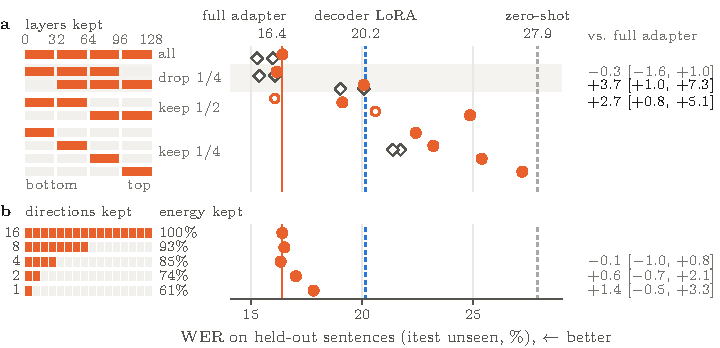
\includegraphics{figs/layers_rank.pdf}
\caption{\textbf{The read-speech gain needs the bottom quarter of the 7B encoder, not the top one,
and survives truncation to 4 of 16 directions per projection.} Dots: the 7B encoder LoRA (one
seed) zeroed after training (a)~outside the orange quarters or (b)~beyond the top singular
directions. Rings: retrained on those layers only. Diamonds: enc+dec seeds. Right: dot vs.\ full
adapter, 95\% interval, grey if it includes 0.}
\label{fig:layers}
\end{figure}

\paragraph{In the 7B, encoder adaptation improves ranking, not coverage.} It cuts other-word
substitutions on itest unseen from 5.8 to 4.0 WER points, yet enc+dec and v2 reach the same oracle
WER (best of 8 beams; 14.0). On a shared pool of held-out-sentence candidates, the enc+dec
likelihood orders 76.9\% vs.\ 69.7\% of a clip's candidate pairs (different word-error counts)
correctly ($+7.3$ \ci{+3.6}{+11.7}; spontaneous $+1.9$ \ci{+0.4}{+3.5}, descriptive; OOD $+1.2$
\ci{-0.9}{+3.3}): significantly for whole-word differences, not for one-letter contrasts
(/q/-/k/, ejective, aspiration), which the encoders already separate (Fig.~\ref{fig:plasticity}a).

\section{Candidates Are Not the Limit; Verification Is}\label{sec:rl}
\paragraph{Sampling and perturbed audio find better candidates than beam search.} On 150
held-out-sentence clips, a transcript better than v2's top-1 is among 8 beam hypotheses for 6.0\%,
8 samples for 14.0\% and 8 perturbed-audio decodes for 16.7\% of clips (McNemar vs.\ beam
$p{=}0.017$, $0.0025$), in line with NoisyRollout \cite{liu2025noisyrollout} in vision RL.

\paragraph{Choosing among candidates is the limit.} The hybrid orders correctly 71--78\% of
candidate pairs; extra verifiers (e.g.\ a second CTC model, an OmniVoice TTS likelihood) did not
help (for English CTC the oracle gap is linguistic \cite{novosad2026oracle}). Synthetic verifiers
of known accuracy (the hybrid blended toward the oracle; the oracle plus Gaussian noise) map
pairwise accuracy to selection WER. At our accuracy, the noisy oracle matches our WER within its 95\% interval on three of four
sets (not on itest unseen: about 13.5 vs.\ 16.9), so accuracy largely explains our errors; on
these curves, five more points of accuracy would mean 13--50\% lower WER. The enc+dec scorer adds
1.5--2.0 points, and its real WER change ($-0.5$ dev unseen, $-1.4$ itest unseen) falls between
the two families' predictions.

\paragraph{RL on labelled data did not help,} unlike high-resource GRPO \cite{shivakumar2025grpoasr}:
MWER \cite{prabhavalkar2018mwer}, GSPO \cite{zheng2025gspo}, Dr.~GRPO \cite{liu2025drgrpo} and a
cross-entropy control from v2, trained on half of the held-out sentences, changed the other half
by $+0.3$ to $+1.6$ (n.s.); GSPO from enc+dec made OOD worse ($+2.1$ \ci{+0.8}{+3.5}).

\section{Conclusion}
Better candidates are cheap to find; ranking them is the bottleneck, and in the 7B encoder
adaptation helped by ranking better. Lessons: evaluate on held-out sentences when prompts are
reused; adapt the encoder when the decoder lacks the language (Whisper) and, in our model family,
for the 7B; invest in reference-free verification, since our candidate pools already hold much
better transcripts (oracle 8.6 vs.\ our 16.9 on itest unseen, 7.3 vs.\ 13.7 OOD). Compute: two NVIDIA L40S
GPUs; code: \url{https://github.com/Sekinal/simbig2026-puno-quechua-asr}. \emph{Limitations:} no official test scores yet; no labelled elderly speech; 4
and 6 spontaneous dev/itest speakers; one seed for the smaller models and most layer analyses;
the plasticity and decoder-prior explanations are hypotheses. \emph{Ethics:} test data were used under the organizers' data-use agreement; no
speaker identification was attempted. \emph{AI assistance:} Claude Opus 5.5 (Anthropic, via
Claude Code) was used for code, experiments, literature search, writing and figures; all results
come from the released code and were checked by the author, who takes full responsibility.

\begin{credits}
\subsubsection{\ackname} The author thanks Lium for a generous GPU credit grant that funded the
compute for this work.
\end{credits}

\bibliographystyle{splncs04}
\bibliography{refs}
\end{document}
